\capitulo{3}{Conceptos teóricos}

En este proyecto se deben de emplear una gran cantidad de  conocimientos adquiridos a lo largo de las asignaturas del grado. En esta sección se describirán cuales son esos conceptos además de la forma en la que se aplican en este proyecto.

\section{Organización de la infraestructura}

Para la implementación del sistema que nos va a permitir el desarrollo del sistema que tiene como objetivo este proyecto se necesitarán tres elementos principales:
\begin{itemize}
	 \item Láser: esta parte es la que se encarga de obtener los datos de su entorno. Estos datos serán enviados a través de una interfaz hacia la unidad de tratamiento de datos. En este caso, el láser del que se dispone, y por lo tanto con el que se va a desarrollar el proyecto es el Hokuyo Safety Laser Scanner (UAM-05LP-T301). Este aparato es capaz de desarrollar tres áreas de detección dependiendo de la distancia a la que detecte un elemento (puede ser de 20, 10 y 5 metros). Aunque sea este láser con el que se va a realizar el proyecto, el principal objetivo es el de poder hacer que el programa pueda funcionar en diferentes tipos de láser con diferentes formas de obtención de datos.\\
    \item Cable ethernet: es el soporte a través del cual se transportan tanto los mensajes enviado por el ordenador hacia el láser como las respuestas y los datos de lectura que este manda al PC demandante. Esta es la que, en la descripción del anterior elemento se conoce como la interfaz. En el caso de este proyecto se usará un UAM-NET, un cable Ethrernet de 3 metros de longitud desarrollado por Hokuyo, misma empresa desarrolladora del láser empleado, lo que hace que resulte idóneo para evitar problemas de incompatibilidad y asegurar así el correcto funcionamiento del sistema.
    \item PC: es la parte principal del proyecto, ya que es la encargada de permitir al usuario tanto introducir las áreas donde se necesita detectar los objetos, como las órdenes que el usuario desea transmitir al láser para recibir la información. Además también es la encargada de recibir y procesar las respuestas del láser para poder mostrar al usuario los resultados de la comparación de los datos y las coordenadas de las áreas introducidas. La utilización de este aparato es debida a que este proyecto sería destinado a ser introducido dentro de un AGV pero se necesita hacer visible al usuario a través de una pantalla.\\ 
\end{itemize}

\subsection{Implementación final en el AGV}
Con esta estructura, el sistema puede ser implementado en AGVs que no posean movimiento, es decir, aquellos cuyas partes móviles no hagan desplazar toda la estructura del vehículo, ya que se necesita un ordenador para visualizar los resultados del análisis.

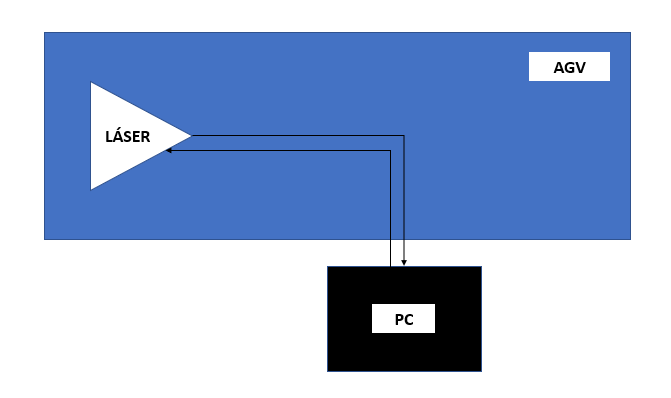
\includegraphics[scale=0.5]{diagrmaExt3}

Esta primera opción de implementación tiene ciertas ventajas pero también posee ciertos inconvenientes:
Ventajas:
\begin{enumerate}
	\item Visualización de la gráfica que representa tanto las lecturas del láser como el resultado del análisis de forma más visual y fácil de analizar por el usuario.
	\item Facilidad para el cambo de coordenadas de cada uno de los límites que conforman cada una de las áreas a analizar.
\end{enumerate}
Desventajas:
\begin{enumerate}
	\item Necesidad de un PC externo que realice el análisis de datos.
\end{enumerate}

Aunque si se obvia esta característica de la detección de objetos (reduciendo ese proceso a datos booleanos) si que es posible emplear el sistema con AVGs móviles.

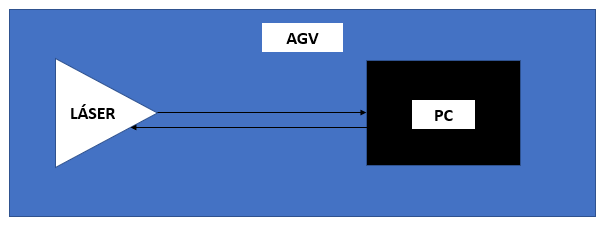
\includegraphics[scale=0.5]{diagrmaInt3}

Aunque esta opción tambien tiene sus ventajas e inconvenientes, al igual que la anterior:
Ventajas:
\begin{enumerate}
	\item Independencia de ningún PC externo que realice el análisis.
	\item Reducción de utilización de recursos (tanto hardware como software) en la ejecución del sistema, debido a la omisión de la representación gráfica.
\end{enumerate}
Desventajas:
\begin{enumerate}
	\item Incapacidad de visualización de los resultados del análisis debido a la ausencia de representación antes mencionada.
\end{enumerate}
\section{Sistemas distribuidos}

Se denomina sistema distribuido a aquel sistema en el que cada equipo se conecta con el resto de los integrantes del sistema para poder compartir sus recursos además de poder utilizar los recursos que comparten el resto de los equipos conectados para realizar procesos para los cuales se necesitan una cantidad de recursos que mayor de la que el usuario de cada equipo posee de forma local. Otra forma de definir este concepto es la ejecución de procesos desde un equipo en otro cuyas características se adapten mejor a las del objetivo que se desea alcanzar.\\
En el caso de este proyecto, la forma en la que se emplea el concepto de sistema distribuido es la que se adapta a la última de las definiciones antes mencionadas. Esto se debe a que el PC se comunica vía cable ethernet con el láser ya que es el único elemento que puede realizar los procesos de lectura de área y devolver al PC los datos correspondientes o, en defecto de estos, el mensaje de error correspondiente.\\
En este caso se establece una estructura de cliente- servidor, siendo cada uno de ellos el PC y el láser respectivamente. Esto se demuestra al observar que el funcionamiento se basa en el envío de comandos desde el PC al láser (petición) y este responde con los datos de lectura o de error (respuesta).

\section{Procesado de datos}

La minería de datos es la ciencia a través de la cual se analiza un gran conjunto de datos para poder descubrir características, patrones o comportamientos ocultos a primera vista.\\
Cuando el programa desarrollado se comunica con el láser, este debe recibir las tramas que el láser crea al analizar su área de observación, las cuales deben de ser tratadas para separar la información importante de las cabeceras y demás datos que el láser usa para interactuar con su aplicación. Una vez hemos conseguido extraer ese tipo de datos, hemos de descartar aquellos datos correspondientes a las zonas donde el láser no detecta ningún objeto, quedándonos solo con aquellas lecturas con valor significativo para la función principal del programa. Tras esto, se analizarán los datos para ver si se encuentran dentro de los límites establecidos por cada una de las áreas a analizar según las preferencias del usuario.\\

\subsection{Comandos disponibles}

Para que el láser devuelva los datos de sus lecturas se le debe de mandar un comando específico dependiendo de la forma de lectura que deseamos que realice. Hay muchos tipos de comandos disponibles para enviar al láser pero para los objetivos de este proyecto vamos a emplear un único tipo, los comandos AR.\\
Estos comandos son los que le indican al láser la orden de enviar los datos de lectura. Dependiendo del comando AR enviado, se enviará un determinado conjunto de datos u otro. Algunos de estos comandos sirven para detener el funcionamiento provocado por otros comandos del mismo tipo. Los comandos de este tipo son 6:
\begin{enumerate}
	\item AR00: envía la medición de las distintas distancias de una única lectura del entorno.
	\item AR01: envía las mediciones de las distintas distancias e intensidades de una única lectura del entorno.
	\item AR02: envía las mediciones de las distintas distancias de cada una de las lecturas del entorno que realiza de forma contínua.
	\item AR03: sirve para detener el comportamiento continuado del comando AR02, se recibe después un mensaje de confirmación.
	\item AR04: envía las mediciones de las distintas distancias e intensidades de cada una de las lecturas del entorno que realiza de forma contínua.
	\item AR05: sirve para detener el comportamiento continuado del comando AR04, se recibe después un mensaje de confirmación.
\end{enumerate} 
 \subsection{Envío y recepción de mensajes}
 Tras haber escogido el comando a utilizar, se debe construir el mensaje que se va a enviar desde el PC hacia el láser. Para esta construcción se debe de seguir una estructura específica basada en estos campos.\\
 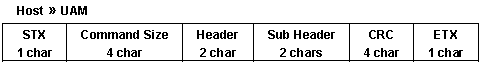
\includegraphics[scale=0.9]{estructuraMsgEnv}
 \begin{itemize}
 	\item STX: Carácter, habitualmente correspondiente a "2" codificado como Bytes, que indica al láser el comienzo del mensaje que se le desea enviar.
 	\item Command size: como su propio nombre indica, es el tamaño del mensaje que el láser va a recibir incluyendo los caracteres de inicio y fin. Para los comandos que se van a emplear en este proyecto, los 4 caracteres que representan esta parte del mensaje van a ser siempre "000E" ya que siempre tienen la misma extensión de 14 caracteres.
 	\item Header: o cabecera, es la parte del mensaje que indica el tipo de comando que se está mandando desde el ordenador. En este caso "AR".
 	\item Subheader: después de haber expresado el tipo de comando, se especifica en te campo que comando del tipo escogido se va a enviar.
 	\item CRC (Cyclical Redundancy Checking):  o verificación de redundancia cíclica, es un código que se añade al mensaje para que e láser verifique la ausencia de fallos en la creación o transmisión del mensaje recibido. Existen muchos tipos de CRC, pero en el caso del láser empleado se usa el CRC Kermit.
 	\item EXT: Carácter, habitualmente correspondiente a "3" codificado como Bytes, que indica al láser el final del mensaje que se le desea enviar.
 \end{itemize}
 
Tras recibir este mensaje, el láser analiza este mensaje, para comprobar que no falte ninguna de las partes descritas anteriormente y la corrección del CRC (evitando fallos de trasmisión). El mensaje de respuesta también obedece a una estructura muy estricta:\\
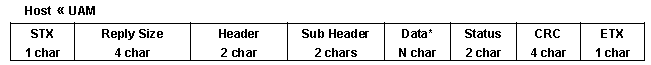
\includegraphics[scale=0.9]{estructuraMsgRcv}
\begin{itemize}
	\item STX y ETX: Son los caracteres de inicio y final del mensaje enviado pro el láser. su definición es identica a la de sus homólogos en el anterior mensaje descrito.
	\item Reply size: al igual que en el anterior se especifica el tamaño del mensaje en 4 caracteres que representan este valor en hexadecimal aunque a diferencia con esta, este tamaño si que es variable ya que no siempre se van a mandar la misma cantidad de datos.
	\item Header y Subheader: son la cabecera y el número del comando recibido por el láser en el anterior mensaje. Sirve de confirmación al usuario de la correcta comprensión del láser a cerca del comando enviado.
	\item Data: como indica su nombre, son los datos de las lecturas realizadas por el láser. Este campo es el único en toda la comunicación el cual no es obligatorio ya que hay casos en los que se puede omitir. Se destacan dos casos:
	\begin{itemize}
		\item Mensaje de error: en los mensajes de error (cuando alguna de las comprobaciones no se ha verificado o la lectura realizada por el láser no se ha terminado con éxito) este campo se omite ya que no hay datos a enviar.
		\item Comandos continuos: en los comandos que provocan un comportamiento de lectura del láser contínua (AR02 o AR04) se envía primero un mensaje con la respuesta que se está describiendo y después se envian mensajes sucesivos (con el mismo comienzo y fin que los otros) donde se muestran los datos.
	\end{itemize}
	\item Status: es el estado del mensaje. A no ser que el mensaje sea un mensaje de error, el resto debería de ser "00" o similar. En caso de que sea un error, estos dos caracteres cambiarán dependiendo del error que ocurra.
	\item CRC: es el código de verificación que demuestra que no ha habido errores en la transmisión, de forma identica a su homólogo en el mensaje enviado en la otra dirección.
\end{itemize}
En el comando empleados en este proyecto (AR02) la forma que posee estos mensajes de respuesta es la siguiente:\\
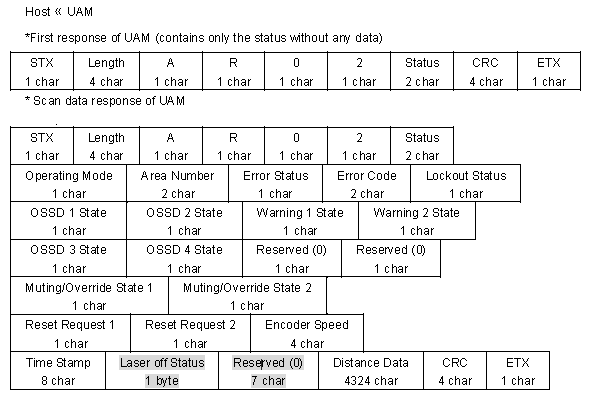
\includegraphics[scale=0.9]{respCorrAR02}
Como se puede observar, dentro del mensaje que posee los datos de las lecturas se pueden encontrar una grán cantidad de datos que indican otra información relevante sobre la lectura realizada aunque irrelevante para los objetivos de este proyecto, como puede ser el estado de las áreas predeterminadas, los estados de alguno de los puertos de salida, el tiempo que se ha tardado en realizar la lectura, etc.\\
Por todo esto se debe analizar cada trama para extraer la parte en la que exclusivamente aparecen los datos, los cuales después se deben traducir.

\subsection{Traducción de los datos}

Después de haber aislado los datos y haberlos dividido en sus correspondientes partes (ya que cada lectura de entorno es enviada por el láser como una cadena de gran longitud) se debe traducir cada uno de los datos (que posee una longitud de 4 caracteres lo cual se deduce de los 4324 caracteres recibidos divididos entre las 1081 lecturas realizadas por cada lectura de entorno del láser) según una serie de pasos a seguir:
\begin{enumerate}
	\item Se extra el equivalente en hexadecimal de cada uno de los 4 caracteres.
	\item Si el dato hexadecimal está entre los $30_{h}$ y  $39_{h}$, se le resta  $30_{h}$. Por le contrario, si el dato se encuentra entre los  $41_{h}$ y  $46_{h}$, se le resta $37_{h}$.
	\item Se traduce cada dato transformado a codificación binaria.
	\item El comjunto de caracteres binarios transformados en una cadena conjunta se traduce a decimal para extraer el dato expresado en milímetros.
\end{enumerate}
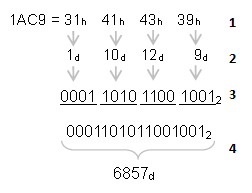
\includegraphics[scale=0.9]{decodeData}